\section{Proposed System Architecture}

\begin{figure*}[t]
\centering
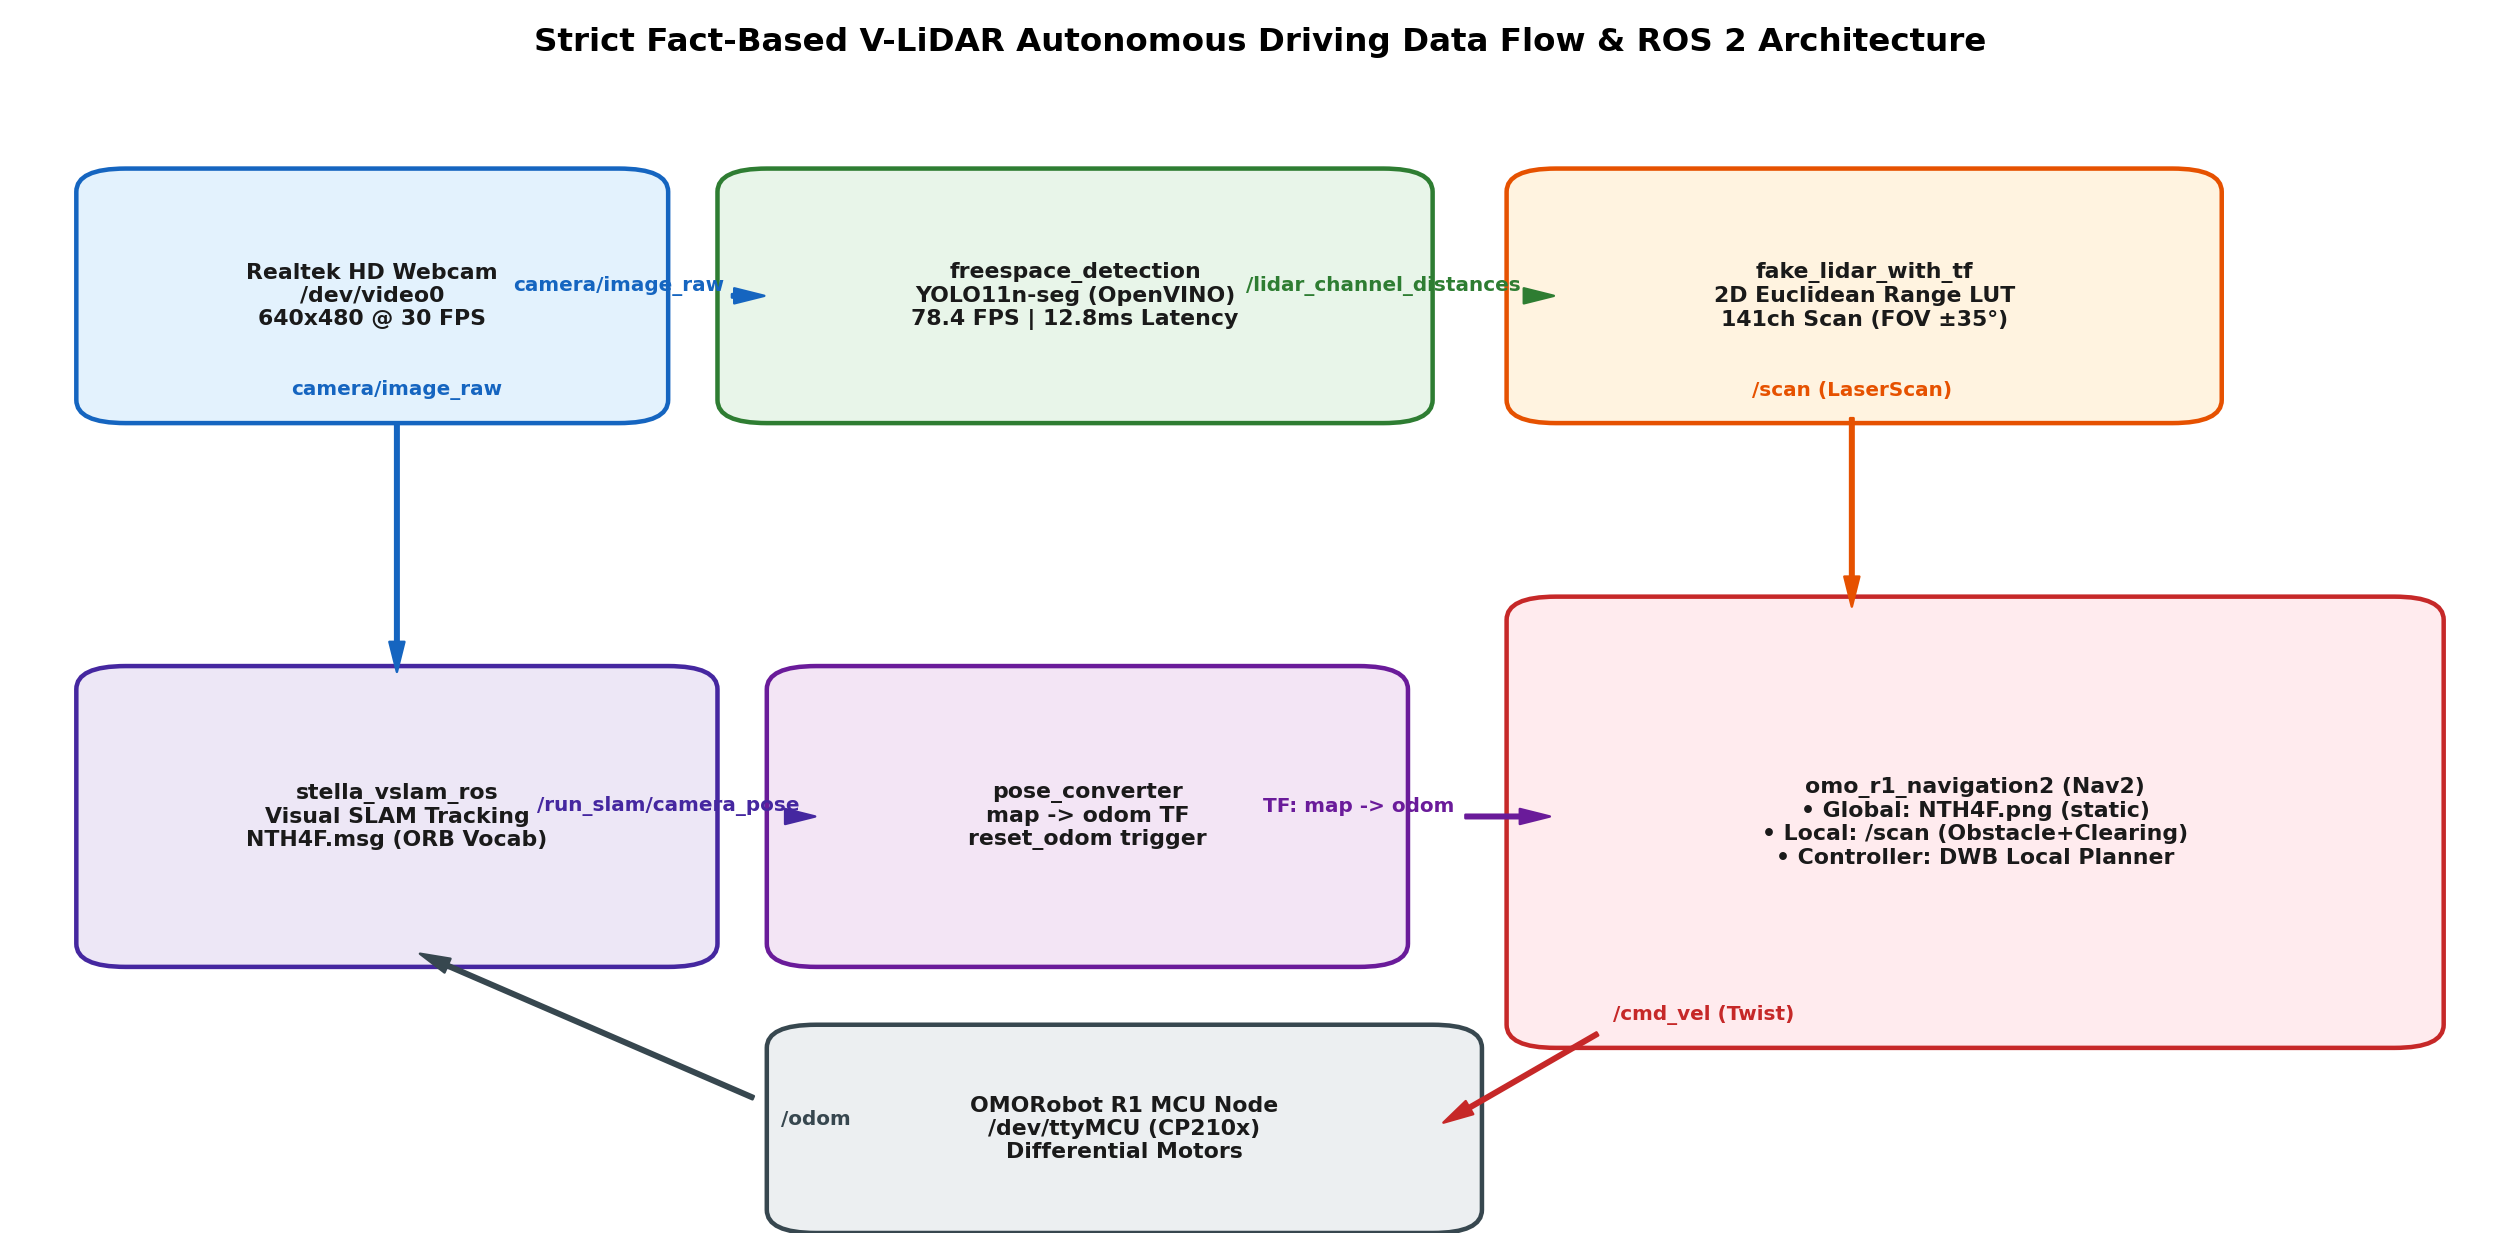
\includegraphics[width=0.92\textwidth]{figures/fig1_v_lidar_pipeline.png}
\caption{System architecture of the proposed Vision-Based 2D Scan Generation (V-LiDAR) framework and its seamless integration with the ROS 2 Nav2 navigation stack.}
\label{fig:pipeline}
\end{figure*}

The architecture of our proposed V-LiDAR system is illustrated in Fig.~\ref{fig:pipeline}. The complete pipeline comprises three interconnected modules: (i) real-time monocular floor segmentation, (ii) geometric Look-Up Table (LUT) range projection, and (iii) ROS 2 Nav2 costmap marking and raytracing.

\subsection{Real-Time Semantic Floor Segmentation}
A forward-facing monocular USB camera mounted on the robot acquires RGB images at $30\,\text{fps}$. To achieve real-time inference on edge computing hardware (e.g., Intel NUC / Jetson), we fine-tuned the ultra-compact \texttt{YOLOv11n-seg} model~\cite{ultralytics2024yolo11}. Frames are downsampled to $256 \times 256$ pixels. The network outputs a binary segmentation mask $M(x, y) \in \{0, 1\}$, where $M(x, y) = 1$ denotes traversable free floor space, and $M(x, y) = 0$ denotes non-floor regions (obstacles, walls, furniture).

\subsection{Geometric Formulation and Look-Up Tables (LUTs)}
Rather than evaluating nonlinear inverse camera projections on every frame, our system precomputes two static Look-Up Tables based on calibrated extrinsic and intrinsic camera parameters:
\begin{itemize}
    \item Camera mounting height: $H = 1.05\,\text{m}$
    \item Downward tilt pitch angle: $\theta = 2.0^\circ$
    \item Vertical Field of View (V-FOV): $\alpha_v = 47.48^\circ$
    \item Horizontal Field of View (H-FOV): $\alpha_h = 70.0^\circ$
\end{itemize}

\subsubsection{Column-to-Bearing Mapping}
For each image column $x \in [0, W-1]$, the relative horizontal azimuth angle $\phi(x)$ with respect to the robot optical center $c_x$ is computed as:
\begin{equation}
    \phi(x) = \arctan\left(\frac{x - c_x}{f_x}\right)
\end{equation}
where $f_x$ is the horizontal focal length. The system discretizes the $70^\circ$ horizontal span into $N = 141$ angular sectors spaced by $\Delta \phi = 0.5^\circ \approx 0.00873\,\text{rad}$, mapping each column into its corresponding scan sector index $k \in [0, 140]$.

\subsubsection{Row-to-Range Mapping}
Under the flat-ground assumption ($Z_{\text{world}} = 0$), each image row $y \in [0, H_r-1]$ corresponds to a ray depressed at angle $\theta(y)$ below the horizontal plane:
\begin{equation}
    \theta(y) = \theta + \arctan\left(\frac{y - c_y}{f_y}\right)
\end{equation}
where $c_y$ and $f_y$ denote the vertical principal point and focal length, respectively. The metric ground distance $d(y)$ from the camera origin to the ground intersection is deterministically given by:
\begin{equation}
    d(y) = \frac{H}{\tan(\theta(y))}
\end{equation}
These metric values are pre-stored in a 1D lookup array, ensuring instant $O(1)$ query time per pixel during runtime.

\subsection{Obstacle Contact Point Extraction and Scan Synthesis}
In each sector column $k$, the algorithm scans upward from the bottom row ($y = H_r - 1$). The lowest non-floor pixel ($M(x, y) = 0$) marks the physical boundary where the obstacle rests on the floor plane. The corresponding distance $d(y)$ is assigned as the range reading for channel $k$. If an entire column consists purely of traversable floor ($M(x, y) = 1$ throughout), the channel is marked as maximum range ($d_{\text{max}} = 10.0\,\text{m}$).

The resulting array of 141 range readings is packaged into a standard ROS 2 \texttt{sensor\_msgs/LaserScan} message published on the \texttt{/scan} topic at $10\,\text{Hz}$.

\subsection{ROS 2 Nav2 Costmap Integration}
The published virtual scan is directly consumed by the Nav2 local costmap obstacle layer~\cite{macenski2020marathon}. Points within valid range thresholds mark obstacle cells as occupied (cost 254), while clear floor lines trace rayclearing lines to erase stale obstacles. A dynamic ROI-based visibility filter further purges phantom obstacle artifacts when the frontal path remains clear for multiple consecutive frames.
